% Data flow diagram
% Author: David Fokkema
\documentclass{article}
\usepackage[margin=0.5in]{geometry}
\usepackage{mathtools}
\usepackage{tikz}
\usetikzlibrary{arrows}

% Modified from http://www.texample.net/tikz/examples/data-flow-diagram/

\begin{document}
\begin{figure}
\centering
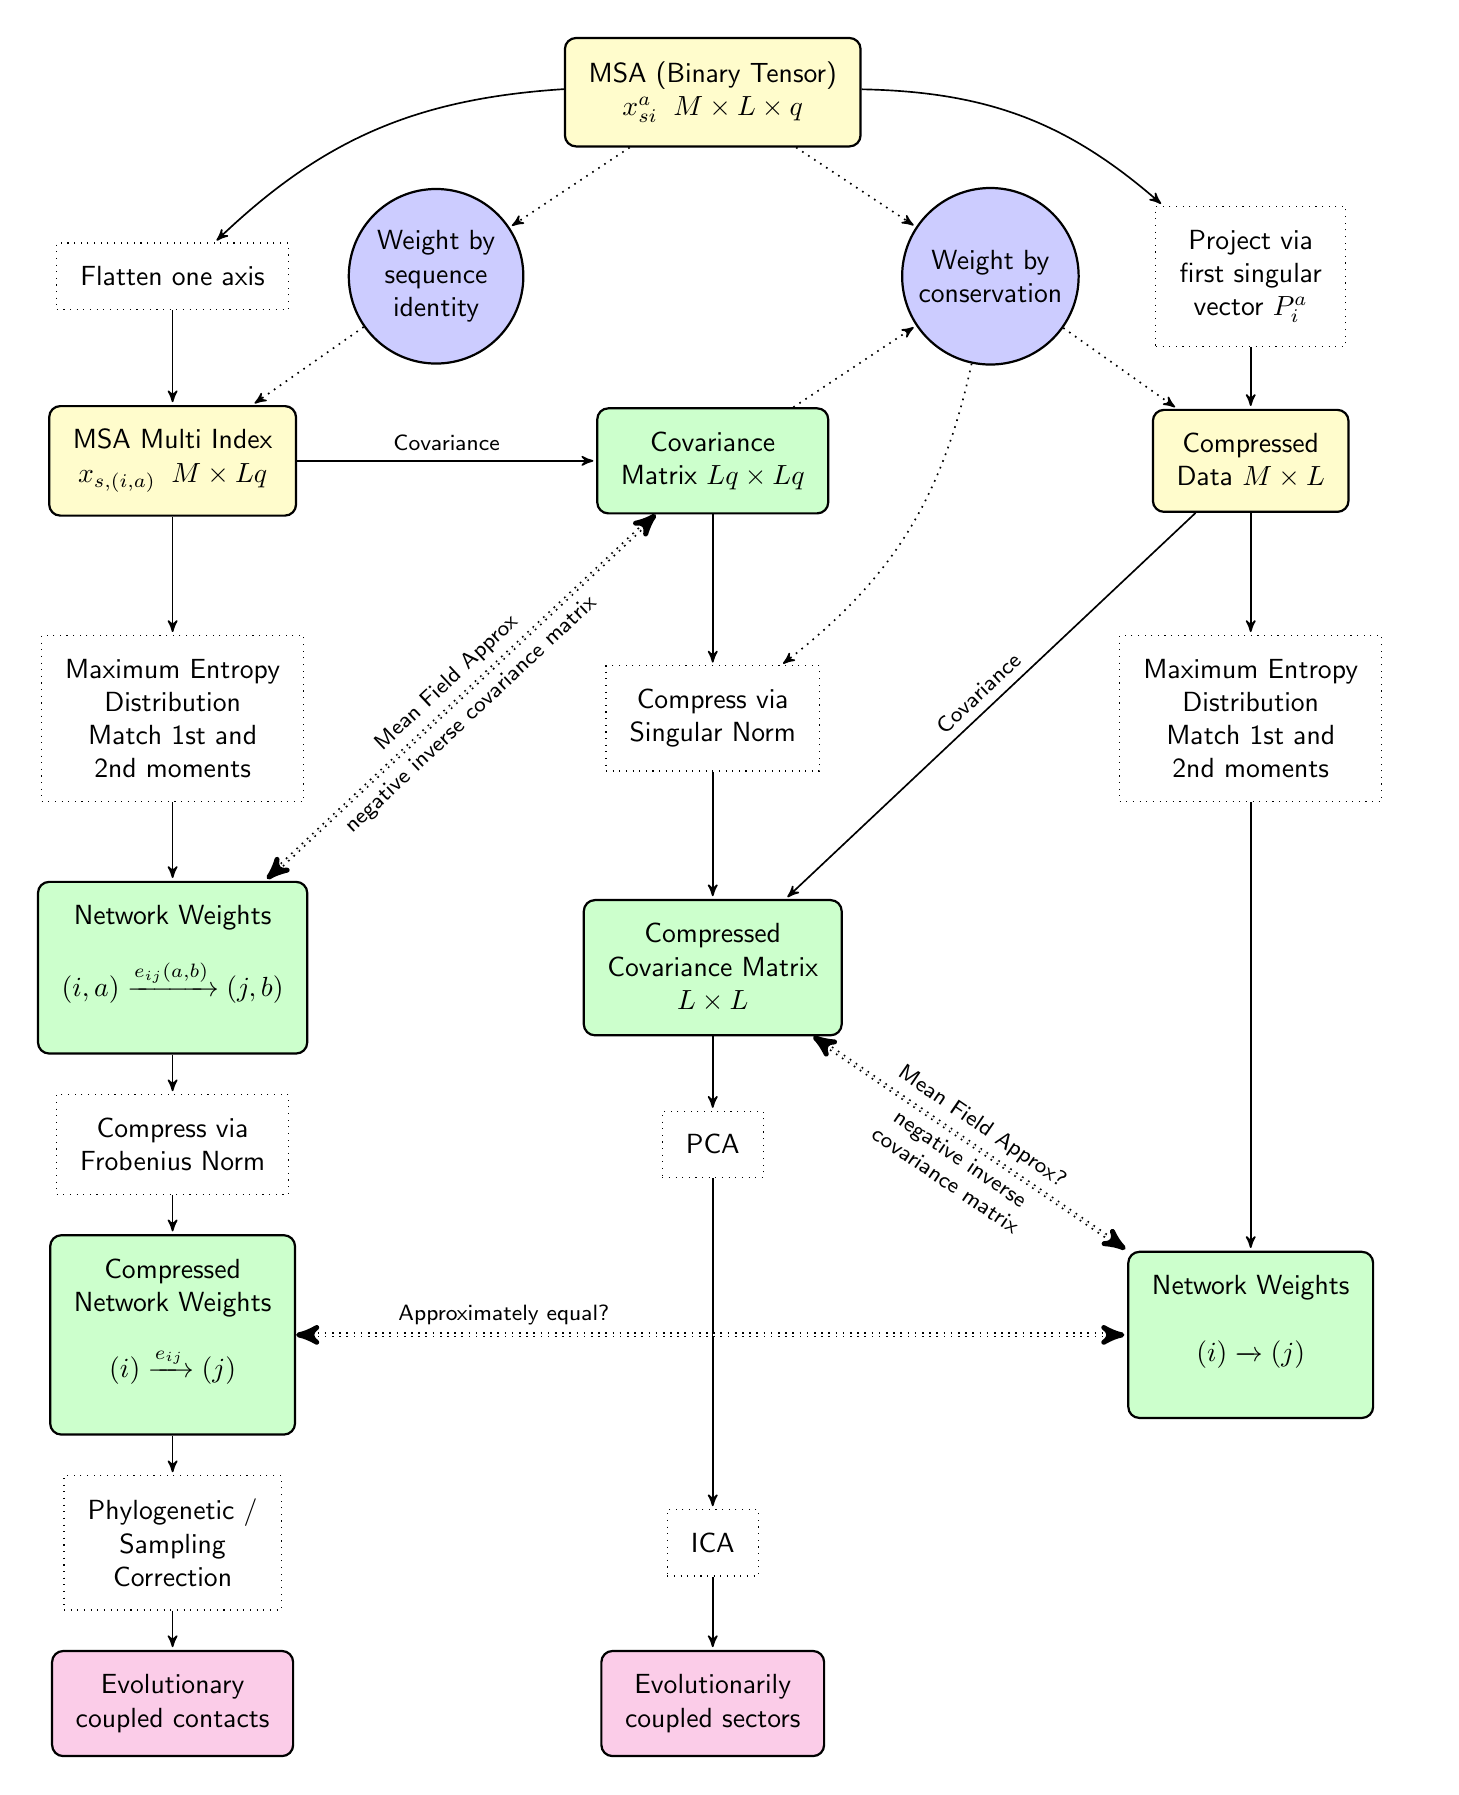
\begin{tikzpicture}[
  font=\sffamily,
  every matrix/.style={ampersand replacement=\&,column sep=.5cm,row sep=.5cm},
  datamat/.style={draw,thick,rounded corners,fill=yellow!20,inner sep=.3cm},
  process/.style={draw,thick,circle,fill=blue!20},
  calcmat/.style={datamat,fill=green!20},
  calcmatfinal/.style={datamat,fill=magenta!20},
  algoprocess/.style={draw,thin,dotted,inner sep=.3cm},
  to/.style={->,>=stealth',shorten >=1pt,semithick,font=\sffamily\footnotesize},
  todots/.style={->,dotted,>=stealth',shorten >=1pt,semithick,font=\sffamily\footnotesize},
  toapprx/.style={<->,double,dotted,>=stealth',shorten >=1pt,semithick,font=\sffamily\footnotesize},
  every node/.style={align=center}]
% Position the nodes using a matrix layout
  \matrix{

    \&
    \&  \node[datamat] (MSA) {
            MSA (Binary Tensor) \\ $x_{si}^a \; \; M\times L \times q$
        }; 
    \&
    \& \\

    \node[algoprocess] (FlattenAxis) {Flatten one axis}; 
    \& \node[process] (weightseqid) {
                Weight by \\ sequence \\ identity
        }; 
    \& 
    \& \node[process] (weightcons) {
                Weight by \\ conservation
        }; 
    \& \node[algoprocess] (SingularProj)  {
                Project via \\ first singular \\vector $P_i^a$
    }; \\

    \node[datamat] (FlattenMSA) {
            MSA Multi Index \\ $x_{s, (i,a)}\;\; M\times Lq$
        };  
    \& 
    \& \node[calcmat] (CovMat) {
            Covariance\\Matrix $Lq\times Lq$
        };
    \&
    \& \node[datamat] (DataProj) {
            Compressed\\Data $M\times L$
        }; \\

    % new line in matrix
    \\
    \\

    \node[algoprocess] (MaxEntBig) {
            Maximum Entropy \\Distribution\\ Match 1st and \\ 2nd moments
        };  
    \& 
    \& \node[algoprocess] (CompressCov) {
            Compress via\\Singular Norm
        };
    \&
    \& \node[algoprocess] (MaxEntSmall) {
            Maximum Entropy \\Distribution\\ Match 1st and \\ 2nd moments
        };  
    \& \\

    \\

    \node[calcmat] (NetworkBig) {
            Network Weights \\ \\ $(i,a) \xrightarrow{e_{ij}(a,b)} (j,b)$ \\ 
        };  
    \& 
    \&
    \node[calcmat] (CompressCovmat) {
            Compressed \\ Covariance Matrix \\ $L\times L$
        };
    \& \\

    \node[algoprocess] (CompressFrob) {
            Compress via\\ Frobenius Norm
    };
    \&
    \&
    \node[algoprocess] (PCA) {PCA};
    \& \\

    \node[calcmat] (NetworkBigSmall) {
            Compressed \\ Network Weights \\ \\ $(i) \xrightarrow{e_{ij}} (j)$ \\ 
        };  
    \&  
    \&  
    \&     
    \& \node[calcmat] (NetworkSmall) {
            Network Weights \\ \\ $(i) \xrightarrow{} (j)$ \\ 
        };  
    \\

    \node[algoprocess] (APC) {
            Phylogenetic / \\ Sampling \\Correction
        };
    \&  
    \&  
    \node[algoprocess] (ICA) {ICA};
    \&  
    \&   \\


    \node[calcmatfinal] (Contacts) {Evolutionary \\coupled contacts};
    \&  
    \&  
    \node[calcmatfinal] (Sectors) {
            Evolutionarily \\ coupled sectors
    }; 
    \&  
    \&   \\
  };

  % Draw the arrows between the nodes and label them.
  \draw[to]     (MSA) to[bend right=20] 
                (FlattenAxis);
  \draw[to]     (FlattenAxis)       --  (FlattenMSA);
  \draw[to]     (MSA) to[bend left=20]             
                (SingularProj);
  \draw[to]     (SingularProj)      --  (DataProj);
  \draw[todots] (MSA)               --  (weightseqid);
  \draw[todots] (MSA)               --  (weightcons);
  \draw[todots] (weightseqid)       --  (FlattenMSA);
  \draw[to]     (FlattenMSA) to 
                    node[midway,above]{Covariance}
                (CovMat);
  \draw[to]     (DataProj) to 
                    node[midway,above,sloped]{Covariance}
                (CompressCovmat);
  \draw[todots] (CovMat)            --  (weightcons);
  \draw[todots] (weightcons)        --  (DataProj);
  \draw[to]     (FlattenMSA)        --  (MaxEntBig);
  \draw[to]     (CovMat)            --  (CompressCov);
  \draw[todots] (weightcons)    to[bend left=20]  
                (CompressCov);
  \draw[to]     (DataProj)          --  (MaxEntSmall);
  \draw[to]     (MaxEntBig)         --  (NetworkBig);
  \draw[to]     (MaxEntSmall)       --  (NetworkSmall);
  \draw[to]     (NetworkBig)        --  (CompressFrob);
  \draw[to]     (CompressCov)       --  (CompressCovmat);
  \draw[to]     (CompressCovmat)    --  (PCA);
  \draw[to]     (PCA)               --  (ICA);
  \draw[toapprx](CompressCovmat)    to
                    node[midway,above,sloped] {Mean Field Approx?} 
                    node[midway,below,sloped] {
                            negative inverse \\covariance matrix
                    } 
                (NetworkSmall);
  \draw[to]     (ICA)            --  (Sectors);
  \draw[toapprx](NetworkBigSmall)   to
                    node[near start,above,sloped]{Approximately equal?}
                (NetworkSmall);
  \draw[toapprx](CovMat)        to 
                    node[midway,above,sloped] {Mean Field Approx} 
                    node[midway,below,sloped] {
                            negative inverse covariance matrix
                    } 
                (NetworkBig);
  \draw[to]     (CompressFrob)      -- (NetworkBigSmall);
  \draw[to]     (NetworkBigSmall)   -- (APC);
  \draw[to]     (APC)               -- (Contacts);
\end{tikzpicture}
\caption{Right column shows connection between 2013Cocco (left column) and 2016Rivoire (middle column)}
\end{figure}
\end{document}
